% !TeX spellcheck = cs_CZ
%{\tikzset{external/prefix={tikz/MAI/}}
% \tikzset{external/figure name/.add={ch10_}{}}
%---------------------------------------------------------------------------------------------------
% file ppst.tex
%---------------------------------------------------------------------------------------------------
\chapter{Počet Pravděpodobnosti}\label{mai:IchapIII}
\minitoc
  Slovo pravděpodobnost používáme velmi často. Jaký však je jeho přesný význam? Jsme přesvědčeni, 
  že pravděpodobnost výhry ve sportce je velmi malá. Ani pravděpodobnost, že se vyplní předpověď 
  počasí, nepovažujeme mnohdy za výraznou. Přesto je mezi oběma příklady obrovský kvantitativní 
  rozdíl. Zkusme význam pojmu pravděpodobnost ukázat pomocí konkrétních číselných příkladů.
  
  \begin{itemize}
    \item \textbf{Příklad se střelcem}: Sportovní střelec střílí na terč série \num{100} ran. 
          Předpokládejme, že podmínky při střelbě jsou stále stejné. Stejná je zbraň, terč, 
          vzdálenost, povětrnostní podmínky i momentální zdravotní stav střelce. Při hodnocení 
          střelcova „mistrovství“ někdo řekne, že střelec zasáhne terč s pravděpodobností 
          \num{92}\%. Jak tomu rozumět? Znamená to, že v souboru sérií výstřelů jsou velmi časté 
          ty, v nichž zasáhl střelec terč \num{92}-krát. Samozřejmě, není řídké, že se objeví i 
          série s \num{93} nebo \num{94} zásahy, ale také s \num{91} nebo \num{90}. Vyloučen není 
          ani případ s úspěšností \num{96} či \num{88}, a dokonce i stovku bychom mohli zaznamenat. 
          Situace výrazně odlišné od \num{92} zásahů však budou řídké, a to tím více, čím více se 
          úspěšnost série liší od \num{92} oběma směry.
    \item \textbf{Příklad se zmetky}: Koupíte si výrobek u firmy, o které je známo, že vyrábí 
          zmetky s pravděpodobností 0,16\%? Situaci lze posuzovat obdobně jako úspěšnost střelce. 
          Budeme-li například zkoumat série obsahující 1000 výrobků, bude každá z nich obsahovat „v 
          průměru“ 16\% zmetků. Z příkladu se střelcem již zhruba víme, jak posuzovat slovo v 
          průměru.
  \end{itemize}
  
  V této kapitole se budeme pravděpodobnostmi zabývat podrobněji. Zjistíme, že i když se týkají 
  náhodných jevů, platí i pro ně jisté zákonitosti.
    
  \section{Pravděpodobnost}\label{mai:IchapIIIsecI}
    V úvodních příkladech jsme si vyložili, jak intuitivně chápat pojem pravděpodobnost. Jednalo se 
    v nich o posouzení průměrné úspěšnosti ve velkém souboru operací či úkonů prováděných za 
    stejných podmínek, šlo tedy o jakousi „průměrnou“ pravděpodobnost. Nyní definujeme 
    pravděpodobnost matematicky.
    
    \subsection{Co se pravdě podobá — definice pravděpodobnosti}
      Pro definici pravděpodobnosti použijeme pojmu \emph{náhodný pokus}, jehož význam si ukážeme 
      na příkladu. Dobrým příkladem náhodných pokusů je třeba házení mincí, hraní kostkou, výběr 
      karet z balíčku, vidíme-li pouze jejich rub, apod. Budeme třeba házet kostkou. Abychom si 
      situaci zbytečně nekomplikovali, budeme předpokládat, že všechny výsledky hodu kostkou 
      (náhodné pokusy) jsou stejně časté, žádný z nich není nijak preferován\footnote{Kostka by 
      tedy měla být homogenní, plocha, na kterou po hodu dopadne, vodorovná, kvalita povrchu všech 
      stěn kostky stejná (žádná stěna by třeba neměla být natřena lepidlem), apod.}. Počet možných 
      výsledků jednotlivého hodu je \(N = 6\) (kostka má \num{6} stěn, na každé je vyznačen odlišný 
      počet ok, tedy \num{1} až \num{6}). Jednotlivé situace, které mohou nastat, nazýváme 
      náhodnými jevy. Náhodným jevem \(A\) tak může být situace \emph{„padne číslo \num{2}“}, jiným 
      náhodným jevem \(B\) situace \emph{„padne číslo dělitelné třemi“}, apod. Počet situací, kdy 
      výsledek hodu lze hodnotit tak, že určitý jev nastal, označíme \(M\). Například pro jev \(A\) 
      \emph{„padne číslo \num{2}“} je \(M(A)= 1\), pro jev \(B\) \emph{„padne číslo dělitelné 
      třemi“} je \(M(B) = 2\) (počet ok \num{3} nebo \num{6}). Můžeme také definovat jev \(O\) 
      \emph{„nepadne žádné číslo“} (\(M(0) = 0\)) nebo jev \(J\) \emph{„padne jakékoli číslo“} 
      (\(M(J) = 6\)).
      
      \begin{definition}
        Pravděpodobností jevu rozumíme podíl
        \begin{equation}\label{mai:eq011}
          p = \frac{M}{N} = \frac{\text{počet případů příznivých}}{\text{počet případů možných}}.
        \end{equation}  
        Počtem případů možných jsme zkráceně nazvali počet všech možných výsledků náhodného 
        pokusu, počtem případů příznivých pak počet všech takových výsledků pokusu, při nichž daný 
        jev nastal.
      \end{definition}
      Je zřejmé, že hodnota pravděpodobnosti jakéhokoli jevu je nezáporná a může nabývat hodnoty 
      nejvýše \num{1}, tj. \(0 <p< 1\). Jev s \emph{nulovou pravděpodobností} se nazývá 
      \textbf{nemožný}, jev s \emph{jednotkovou pravděpodobností} je \textbf{jistý}. V našem 
      příkladu s kostkou tak dostáváme
      \begin{equation*}
        p(A) = \frac{1}{6}, \qquad p(B) = \frac{2}{6} = \frac{1}{3}, \qquad
        p(O) = 0, \qquad p(J) = 1.
      \end{equation*}  

      %---------------------------------------------------------------
      % !TeX spellcheck = cs_CZ
\begin{example}
 \label{mai:exam006}
  \textbf{Barevné ponožky}:\newline\small
  V zásuvce jsou ponožky tří barev. Červené (\textbf{Č}), zelené (\textbf{Z}) a modré (\textbf{M}). 
  Je jich tam od každé barvy hodně. Student jde na schůzku a chce si vzít čisté ponožky. Náhle 
  zhasne světlo. Student vytáhne potmě dvě ponožky. Jaká je pravděpodobnost, že ponožky budou mít 
  stejnou barvu? Vyjmenujme případy, které mohou při vytažení dvou ponožek nastat: (\textbf{Č+Č}), 
  (\textbf{Č+Z}), (\textbf{Z+Č}), (\textbf{Č+M}), (\textbf{M+Č}), (\textbf{Z+Z}), (\textbf{Z+M}), 
  (\textbf{M+Z}), (\textbf{M+M}). Je tedy \(n = 9\). Příznivé situace jsou tří, (\textbf{Č+Č}), 
  (\textbf{Z+Z}), (\textbf{M+M}). Pravděpodobnost je tedy 1/3. (Převzato z 
  \cite[s.~200]{Musilova2009MA1}) 
\normalsize
\end{example}
      %---------------------------------------------------------------
    \subsection{Cifry, kostky, karty - kombinatorické opakování}
      Příklad s ponožkami byl velmi jednoduchý. Podařilo se nám vyjmenovat všechny případy možné i 
      všechny případy příznivé, neboť obojího bylo docela málo. Daleko běžnější jsou však situace, 
      kdy výčet případů není schůdný. A tehdy potřebujeme \textbf{kombinatoriku}.
      
      Nechť \(\mathcal{M}\) je \(n\)-prvková množina, z níž budeme provádět výběry \(k\) prvků 
      podle určitých pravidel. Prvky množiny \(\mathcal{M}\) nemusíme nijak konkretizovat. Abychom 
      si však o výběrech a pravidlech pro jejich tvorbu dokázali udělat nějakou názornou představu, 
      je taková konkretizace vhodná. Prvky množiny \(\mathcal{M}\): mohou být třeba žáci ve třídě, 
      barvy, hrací karty, apod. Výběry mohou představovat třeba družstva pro odbíjenou, signály 
      tvořené barevnými praporky, možnosti rozdání karet při mariáši, apod. Jednotlivé typy výběrů 
      získaly své názvy právě na základě pravidel stanovených pro jejich vytváření. Rozhodující 
      jsou dvě základní kritéria:
      \begin{itemize}\addtolength{\itemsep}{-0.5\baselineskip}
        \item Je pro tvorbu výběru podstatné pořadí prvků ve výběru či nikoliv?
        \item Mohou se prvky ve výběru opakovat či nikoliv?
      \end{itemize}
      
      Typy výběrů shrnuje následující diagram:
      \begin{figure}[ht!] %\ref{mai_fig021}
        \centering
        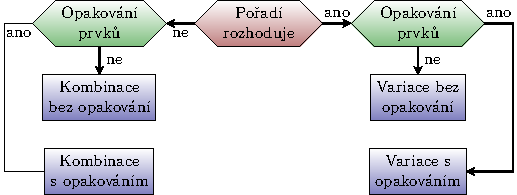
\includegraphics[width=0.7\linewidth]{mai_fig021.pdf}
        \caption{Typy výběrů. \cite[s.~201]{Musilova2009MA1}}
        \label{mai_fig021}
      \end{figure}

      Představuje-li daný výběr například volejbalové družstvo osmi děvčat (šest hráček a dvě 
      náhradnice), které bude reprezentovat v soutěži třídu osmou bé, do níž chodí \num{25} děvčat 
      a \num{18} chlapců, jedná se o výběr \(k — 8\) prvků z počtu \(n = 25\) prvků. Chlapce nelze 
      postavit do družstva volejbalistek. Každý výběr možného družstva bude představovat 
      \emph{kombinaci bez opakování}, neboť pořadí hráček nehraje roli a třeba Aničku Novákovou 
      máme ve třídě jen jednu. Budeme-li však chtít vytvářet z deseti cifer \(0, 1, \ldots, 9\) 
      trojciferná čísla, pak tyto výběry tří prvků z deseti (\(k = 3\), \(n = 10\)) jsou 
      \emph{variacemi s opakováním}. Čísla \num{125}, \num{512}, \num{251}, \num{215}, \num{521} a 
      \num{152} jsou totiž různá, a například \num{222} je také trojciferné číslo. Kombinace s 
      opakováním bychom mohli vytvářet třeba i při výběru různobarevných ponožek ze zásuvky a 
      konečně \emph{variacemi bez opakování} by mohly být dejme tomu trojbarevné signály (\(k = 
      3\)) tvořené trojicemi barevných hadříků vybíraných z \(n\) barev (pro \(n = 3\) třeba zrovna 
      z těch ponožek). Nyní bychom však rádi věděli, jak pro zadané hodnoty \(n\) a \(k\) určit 
      počet všech možných výběrů předepsaného typu. Ukážeme si to na příkladech.

      %---------------------------------------------------------------
      % !TeX spellcheck = cs_CZ
\begin{mdframed}[style=mdexam]
  \begin{example}\label{mai:exam007}
    \textbf{Šance milion}:\newline
    „Znáte nějakou jinou hru, kde můžete denně vyhrát milion?“ Tento nebo jiný, obdobně nepříliš
    vtipný reklamní slogan propaguje v televizi hru, jejímž cílem je uhodnout šestici tažených cifer
    ve správném pořadí. (Hru raději nehrajte, pravděpodobnost výhry je mizivá.) Tah se provádí
    následovně: V každém ze šesti bubnů, očíslovaných pořadovými čísly \num{1} až \num{6}, je
    připraveno deset míčků opatřených ciframi \(0, 1, \ldots, 9\). Z prvního bubnu se náhodně
    vylosuje jedna cifra (deset možností). Poté se náhodně vylosuje jedna cifra z druhého bubnu
    (opět deset možností). Možností vzniku uspořádané dvojice cifer (jedna cifra z prvního a druhá z
    druhého bubnu) je již sto (každou možnost výsledku u prvního bubnu lze kombinovat s každou
    možností výsledku z druhého bubnu). Losování pokračuje u třetího, čtvrtého, pátého a šestého
    bubnu. Celkový počet možností je \num{1e6}, tedy \textbf{milion}. (Šance získat výhru, tedy
    vyhrát milion, je ovšem pouze jedna milióntina, neboť z milionu možností je pouze jedna skutečně
    tažena.) 
  \end{example}
\end{mdframed}
      %---------------------------------------------------------------
      
      Zobecněním předchozího příkladu získáváme vzorec pro počet \textbf{variací s opakováním} 
      \emph{k}-té třídy z \(n\) prvků. Při tahu totiž záleží na pořadí bubnů a každý buben obsahuje 
      všechny cifry. Výsledky tahů z jednotlivých bubnů se tedy mohou opakovat. Pokud by bubnů bylo 
      \(k\) a v každém \(n\) různých cifer, dostali bychom pro \textbf{variace s opakováním 
      \(k\)-té třídy z \(n\) prvků} celkový počet
      \begin{equation}\label{mai:eq007}
        \boxed{V_k' = n^k}\, .
      \end{equation}

      %---------------------------------------------------------------
      % !TeX spellcheck = cs_CZ
\begin{example}\label{mai:exam008}
  \textbf{Modifikovaná šance milion}:\newline
  Představme si hru z předchozího příkladu upravenou takto: K dispozici bude jen jeden buben s 
  ciframi \(0, 1, \ldots, 9\), každá cifra je v bubnu obsažena pouze jednou. Opět máme losovat 
  uspořádanou \textbf{šestici cifer}. Nyní se však jedná o \textbf{variace šesté třídy z deseti 
  prvků bez opakování}. S jediným bubnem musíme totiž provést šest losování, přičemž při každém 
  losování ubude z bubnu jedna cifra. Při prvním tahu je deset možností, při druhém již jen devět, 
  atd., při šestém již pouze pět možností. Celkem je tedy \(10 \cdot 9 \cdots 5 = \num{151200}\) 
  možností.
\end{example}
      %---------------------------------------------------------------
      
      Uvážíme-li, že v předchozím příkladu je \(n = 10\) a \(k = 6\), dostáváme pro \textbf{počet 
      variací bez opakování \(k\)-té třídy z \(n\) prvků} obecný vztah
      \begin{align}
        V_k(n) &= n(n-1)(n-2)\cdots(n-k+1)  \nonumber \\
        \shortintertext{neboli}
        V_k(n) &= \frac{n!}{(n-k)!}\, .    \label{mai:eq008}
      \end{align}
      Poznamenejme, že \(n!\) značí \textbf{faktoriál}, \(n! = n(n — 1)\cdots 3 \cdot 2 \cdot 1\). 
      Pro nulu definujeme \(0! = 1\). Je zřejmé, že při vytváření variací bez opakování musí být 
      \(k\leqq n\). Variace bez opakování \(n\)-té třídy z \(n\) prvků se nazývají 
      \textbf{permutace}. Každá z nich představuje určité uspořádání těchto \(n\) prvků. Platí
      \begin{equation}\label{mai:eq009}
        \boxed{P(n) = V_n(n) = n!}\, .
      \end{equation}
      
      Nyní odvodíme vzorec pro počet \textbf{kombinací \(k\)-té třídy z \(n\) prvků bez opakování}. 
      Již jsme si řekli, že \emph{kombinací} rozumíme takový výběr z celkového počtu \(n\) prvků, 
      který obsahuje určitých \(k\) prvků nezávisle na jejich pořadí. Představme si, že máme k 
      dispozici všechny variace bez opakování \(k\)-té třídy ze zmíněných \(n\) prvků. Vezměme 
      kteroukoli z nich. Soubor všech variací \(k\)-té třídy z \(n\) prvků však obsahuje i další 
      variace, lišící se od té naší jen pořadím prvků. Celkem je takových variací (i s tou první) 
      \(k!\) a z hlediska kombinací představují totéž. Soubor variací se tak rozpadá na podsoubory, 
      z nichž každý obsahuje \(k!\) variací lišících se navzájem pouze pořadím prvků. Každý z 
      těchto podsouborů představuje však jedinou kombinaci. Počet kombinací \(k\)-té třídy z \(n\) 
      prvků bez opakování je tedy
      \begin{equation}\label{mai:eq010}
        \boxed{C(k) = \frac{V_k(n)}{P(k)} = \frac{n!}{(n-k)!\,k!} = 
               \begin{pmatrix}
                n \\
                k
               \end{pmatrix}}\, .
      \end{equation}
      
      Pro odvození vzorce pro \textbf{kombinace s opakováním} použijeme opět příkladu.
      %---------------------------------------------------------------
      % !TeX spellcheck = cs_CZ
\begin{mathexam}{Kuličky v přihrádkách}{exam009}
  Máme kuličky \(n\) různých barev, v každé barvě máme tolik kuliček, kolik bude potřeba. Naším
  úkolem je vytvářet výběry \(k\) kuliček. Na \textbf{pořadí barev nezáleží}, kuliček jedné barvy
  může být ve výběru libovolný počet \(0\leqq s \leqq k\). Výběry budeme vytvářet tak, že budeme
  kuličky dávat do \(n\) přihrádek, z nichž každá bude vyhrazena pro určitou barvu. Pokud tedy v
  daném výběru zrovna nebude třeba modrá kulička, bude přihrádka vyhrazená pro modrou barvu prázdná.
  Budou-li v daném výběru právě tři červené kuličky, budou umístěny v přihrádce vyhrazené pro
  červenou barvu. Vidíme, že pokud konkrétním přihrádkám přisoudíme konkrétní barvy, samotné kuličky
  by již barevné být nemusely, stačily by třeba kuličky skleněné, bezbarvé. Zůstane-li například
  přihrádka pro modrou barvu prázdná, víme, že daný výběr neobsahuje modrou barvu. Budou-li v
  přihrádce pro červenou barvu tři (bezbarvé) kuličky, víme, že daný výběr obsahuje červenou barvu
  třikrát. Příklad takové situace ukazuje následující schéma:
  
  {\centering
    \luafigure[0.9]{mai_fig033.pdf}
    \par}

  Náš úkol můžeme přeformulovat takto: Je třeba rozmístit \(k\) kuliček do \(n\) přihrádek. V každé
  přihrádce může být obecně \(s\) kuliček, kde \(0\leqq s \leqq k\), přitom celkový počet kuliček
  musí být samozřejmě stále \(k\). Můžeme si představit, že \(k\) kuliček máme položených v řadě na
  polici mezi dvěma pevnými stěnami (krajní svislé čáry v předchozím schématu) a různé způsoby
  rozmístění kuliček do přihrádek provádíme přemísťováním pohyblivých přepážek. Kdybychom například
  v předchozím schématu přesunuli druhou svislou čáru, počítáno zleva, až za první kuličku v
  přihrádce na červenou barvu, dostaneme uspořádání, při němž je v přihrádce na modrou barvu jedna
  kulička a v přihrádce na červenou barvu dvě kuličky. Tedy takto:

  {\centering
    \luafigure[0.9]{mai_fig034.pdf}
  \par}

  Mezi dvěma krajními pevnými stěnami máme tedy k dispozici \(k\) pozic pro kuličky a \((n - 1)\)
  pozic pro pohyblivé přepážky. Celkem tedy \((n + k - 1)\) pozic, na které můžeme libovolně
  rozmísťovat \(k\) kuliček a \((n - 1)\) přepážek. Do těchto \((n + k - 1)\) pozic můžeme umístit
  \(k\) kuliček \(C_k'(n)\) způsoby, kde
  \begin{equation}\label{MAI:eq011}
    \boxed{C_k'(n) =  \binom{n + k - 1}{k} = \binom{n + k - 1}{n -1}}\, .
  \end{equation}
  Na zbylé pozice již musíme umístit přepážky. Nebo naopak, nejprve umístíme \((n - 1)\) přepážek a
  potom kuličky. Výsledek je stejný, jak je vidět z předchozího vzorce. Protože jsme vytváření
  kombinací s opakováním \(k\)-té třídy z \(n\) prvků převedli na úlohu o rozmísťování kuliček do
  přihrádek, udává získaný vzorec právě počet takových kombinací. Aby měl vzorec smysl, musí platit
  \(n + k - 1 \geqq k\), tedy \(n \geqq 1\).

  Komu nevyhovuje představa kuliček v přihrádkách a má raději čísla, může uvažovat následovně: Tak
  jako je každé číslo v desítkové soustavě zapsáno pomocí cifer \(0, 1, 2, \ldots , 8, 9\), je k
  jeho zápisu ve dvojkové soustavě potřeba pouze dvou cifer, nuly a jedničky. Představme si nyní
  přepážku jako jedničku a kuličku jako nulu. Náš úkol zjistit počet všech možných způsobů rozdělení
  \(k\) kuliček do \(n\) přihrádek, ohraničených \((n+1)\) přepážkami, můžeme převést na
  ekvivalentní problém: Kolik dokážeme najít čísel, která jsou ve dvojkové soustavě zapsána právě
  \(k\) nulami a \((n + 1)\) jedničkami, požadujeme-li, aby první i poslední cifrou byla jednička?
  Odpověď je jednoduchá. Máme k dispozici \((n+k+1)\) pozic pro cifry. První a poslední pozice jsou
  pevně obsazeny jedničkami, volných pozic je tedy pouze \((n + k - 1)\). Počet všech různých
  způsobů, kterými na \(k\) z těchto pozic můžeme umístit nuly, je roven počtu kombinací \(k\)-té
  třídy z \((n + k - 1)\) prvků. Na zbylé pozice již musíme umístit jedničky. Komplementárně,
  budeme-li hledat počet všech možných způsobů, jak na \((n-1)\) pozic umístit jedničky, dostaneme
  shodný výsledek, v souhlasu se vzorcem (\ref{mai:eq010}).
\end{mathexam}
      %---------------------------------------------------------------
      
      Komu nevyhovuje představa kuliček v přihrádkách a má raději čísla, může uvažovat následovně: 
      Tak jako je každé číslo v desítkové soustavě zapsáno pomocí cifer \(0, 1, 2, \ldots , 8, 9\), 
      je k jeho zápisu ve dvojkové soustavě potřeba pouze dvou cifer, nuly a jedničky. Představme 
      si nyní přepážku jako jedničku a kuličku jako nulu. Náš úkol zjistit počet všech možných 
      způsobů rozdělení \(k\) kuliček do \(n\) přihrádek, ohraničených \((n+1)\) přepážkami, můžeme 
      převést na ekvivalentní problém: Kolik dokážeme najít čísel, která jsou ve dvojkové soustavě 
      zapsána právě \(k\) nulami a \((n + 1)\) jedničkami, požadujeme-li, aby první i poslední 
      cifrou byla jednička? Odpověď je jednoduchá. Máme k dispozici \((n+k+1)\) pozic pro cifry. 
      První a poslední pozice jsou pevně obsazeny jedničkami, volných pozic je tedy pouze \((n + k 
      — 1)\). Počet všech různých způsobů, kterými na \(k\) z těchto pozic můžeme umístit nuly, je 
      roven počtu kombinací \(k\)-té třídy z \((n + k — 1)\) prvků. Na zbylé pozice již musíme 
      umístit jedničky. Komplementárně, budeme-li hledat počet všech možných způsobů, jak na 
      \((n—1)\) pozic umístit jedničky, dostaneme shodný výsledek, v souhlasu se vzorcem 
      (\ref{mai:eq010}).
      
      %---------------------------------------------------------------
      % !TeX spellcheck = cs_CZ
\begin{example}\label{mai:exam010}
  \textbf{Obsazování kvantových stavů}:\newline\small
  Úloha o kuličkách a přihrádkách má přímou aplikaci v \textbf{kvantové fyzice}. Představme si, že 
  fyzikální soustava je tvořena \(k\) částicemi. Každá částice se nachází v určitém stavu, v němž 
  jí můžeme přisoudit fyzikální charakteristiky, které jsou s tímto stavem spojeny (třeba energii, 
  moment hybnosti, apod.). Jednotlivé stavy jsou pak rozlišitelné právě pomocí těchto 
  charakteristik. Dejme tomu, že přípustných stavů je \(n \geqq 1\). Problémem kvantové fyziky je 
  to, že kvantové částice jsou nerozlišitelné. Nepoznáme jednu od druhé. Je to stejné, jako bychom 
  měli \(k\) naprosto stejně vypadajících kuliček, které nemáme nijak očíslovány. Záměna dvou 
  částic (nerozlišitelných kuliček) se nepozná, nevede tedy ke změně stavu fyzikální soustavy. Pro 
  hodnoty fyzikálních charakteristik soustavy jako celku je tedy důležité jen to, kolik částic je v 
  každém z přípustných stavů. Musíme se tedy zajímat o to, kolika způsoby lze našich \(k\) 
  \textbf{nerozlišitelných částic} (kuliček) umístit do \(n\) \textbf{stavů} (přihrádek). Kvantové 
  částice jsou však dvojího druhu, \textbf{fermiony} (například elektrony, neutrony, protony, jádra 
  s lichým počtem nukleonů) a \textbf{bosony} (například fotony, mezony, jádra se sudým počtem 
  nukleonů). Rozdíl mezi nimi je ten, že bosony se „dobře snášejí“, a proto jich může být v jednom 
  stavu i více. 
  \begin{itemize}\addtolength{\itemsep}{-0.5\baselineskip}
    \item Počet možností, jak rozmístit \(k\) \textbf{bosonů} po \(n\) stavech je tedy
          \begin{equation*}
            N_{\text{boson}} = 
              \begin{pmatrix}
                n + k - 1 \\
                    k
               \end{pmatrix}
          \end{equation*}
    \item S \textbf{fermiony} je tomu jinak. \textbf{Pauliho vylučovací princip} jim zakazuje, 
          aby v daném stavu byl více než jeden fermion. Stav může být buď prázdný, nebo obsazen 
          jedním fermionem. V takovém případě musí být \(n \geqq k\) a v každé přihrádce může být 
          nejvýše jedna kulička. Situace tak odpovídá \textbf{kombinacím bez opakování \(k\)-té 
          třídy z \(n\) prvků}, tj.
          \begin{equation*}
            N_{\text{fermion}} = 
              \begin{pmatrix}
                n  \\
                k
              \end{pmatrix}
          \end{equation*}
  \end{itemize}
\normalsize
\end{example}
      %---------------------------------------------------------------
      
      Získané kombinatorické vzorce nyní použijeme při řešení základních úloh o pravděpodobnostech. 
      V každé úloze bude důležité
      \begin{itemize}
        \item definovat jev \(A\), jehož pravděpodobnost počítáme,
        \item určit počet \(N\) případů možných, tj. počet všech možných výsledků pokusu, při 
              kterém sledujeme, zda jev \(A\) nastal či nenastal,
        \item určit počet \(M\) případů příznivých, tj. počet těch výsledků daného pokusu, při 
              kterých jev \(A\) nastal.
      \end{itemize}

      %---------------------------------------------------------------
      % !TeX spellcheck = cs_CZ
\wikitextrule
\begin{example}\label{mai:exam052}
  \textbf{Výhra ve sportce}\newline\small
  Jaká je pravděpodobnost hlavní výhry ve sportce? Všichni víme, že malá, ale máme představu, jak 
  malé toto číslo je? Při sportce se losuje \(k = 6\) čísel a jedno dodatkové z celkového počtu \(n 
  = 49\) čísel. (Dříve byla čísla spojena s názvy sportů, odtud název „sportka“ .) Na pořadí čísel 
  ve výběru nezáleží, vytažené číslo se do hry nevrací. Jde tedy o \textbf{kombinace bez 
  opakování}. Hlavní výhra požaduje uhodnout všech \num{6} tažených čísel. Jev \(A\) je tedy 
  definován takto:
  
  \begin{itemize}
    \item Jev \(A\): Bude taženo právě oněch \num{6} čísel, která jsem vsadil.
          Počet možností, které při tahu sportky mohou nastat (počet případů možných), je \(N = 
          \begin{pmatrix} n \\ k\end{pmatrix} =  \begin{pmatrix} 49 \\ 6 \end{pmatrix} \). Hlavní 
          výhru představuje jediná kombinace, počet příznivých případů je proto \(M = 1\). 
          Pravděpodobnost hlavní výhry ve sportce, tj. pravděpodobnost jevu \(A\), je
          \begin{equation*}
            p(A) = \dfrac{M}{N} = \dfrac{1}{\begin{pmatrix} 49 \\ 6 \end{pmatrix}} 
                 = \dfrac{43!6!}{49!} = \dfrac{720}{49\cdot48\cdot47\cdot46\cdot45\cdot44} \simeq 
                 \num{7e-8}
                 = \SI{7e-6}{\percent}
          \end{equation*}
          Pravděpodobnost hlavní výhry je velmi malá, sedm milióntin procenta. 
    \item A o kolik lepší to bude s pravděpodobností některé z vedlejších výher? Tak třeba pátá 
          cena znamená, že je nutné ze šesti tažených čísel uhodnout libovolné tři. Jev \(A\) je 
          tedy: Ze šesti čísel, která jsme vsadili, budou v tažené kombinaci obsažena právě tři 
          libovolná z nich. Počet \(N\) zůstává stejný jako v předchozí části úlohy. Je třeba jen 
          určit \(M\). Každý příznivý případ vzniká tak, že trojice správných čísel (výběry tří ze 
          šesti) je doplněna trojicí chybných čísel (výběry tří ze čtyřiceti tří). Tedy \(M = 
          \begin{pmatrix}6 \\ 3\end{pmatrix}\begin{pmatrix} 49 - 6 \\ 3\end{pmatrix} =  
          \begin{pmatrix} 6 \\ 3\end{pmatrix}\begin{pmatrix} 43 \\ 3 \end{pmatrix}\),
          \begin{align*}
            p(A) &= \dfrac{M}{N} 
                  = \dfrac{\begin{pmatrix} 6 \\ 3\end{pmatrix}
                           \begin{pmatrix} 43 \\ 3 \end{pmatrix}}
                          {\begin{pmatrix} 49 \\ 6\end{pmatrix} }                
                  =\left(\dfrac{6!}{3!\cdot3!}\right)\left(\dfrac{43!}{40!\cdot3!}\right)
                   \left(\dfrac{43!6!}{49!}\right)                                            \\
                 &=\dfrac{120\cdot43\cdot42\cdot41\cdot720}
                         {49\cdot48\cdot47\cdot46\cdot45\cdot44\cdot36} 
                  \simeq\num{0.018}.
          \end{align*}
          Tato pravděpodobnost již zanedbatelná není, na rozdíl od finanční částky, jíž bývá 
          ohodnocena pátá cena. Sázení sportky může domácímu rozpočtu spíše ublížit.
    \item Třetí, resp. čtvrtá cena jsou, podobně jako první a pátá, definovány velmi jednoduše. Je 
          třeba uhodnout pět, resp. čtyři ze šesti tažených čísel. V případě druhé ceny hraje roli
          dodatkové číslo. Druhou cenu získává ten, kdo uhodl pět ze šesti čísel vylosovaných v 
          prvním tahu a ještě navíc číslo dodatkové, které se losuje ze zbylých \num{43} čísel, jež 
          zůstala po prvním tahu v osudí. Jev \(A\) je tedy definován takto:
          
          Ze šesti čísel, která jsem vsadil, bude při prvním tahu vylosováno libovolných pět a v 
          druhém tahu bude vylosováno právě to dodatkové číslo, které jsem vsadil. Počet případů 
          příznivých je pouze \(M = \begin{pmatrix}6 \\ 5\end{pmatrix}\), neboť šestým číslem 
          nemůže být libovolné ze \num{43} čísel, která nebyla v prvním tahu vylosována, ale 
          musí to být právě číslo dodatkové. Pravděpodobnost jevu \(A\) je
          \begin{equation*}
            p(A)  = \dfrac{M}{N} 
                  = \dfrac{\begin{pmatrix} 6  \\ 5\end{pmatrix}}
                          {\begin{pmatrix} 49 \\ 6\end{pmatrix}}
                  \simeq\num{4.2e-17}.
          \end{equation*}
          
          Pokud bychom jako jev \(A\) označili výhru jakékoliv ceny, dostaneme
          \begin{align*}
            M &= \sum_{6}^{k=3}\begin{pmatrix} 6  \\   k  \end{pmatrix}
                               \begin{pmatrix} 43 \\ 6 - k\end{pmatrix}  +
                               \begin{pmatrix} 6  \\   5  \end{pmatrix}                      \\
              &= \begin{pmatrix} 6 \\ 3\end{pmatrix}\begin{pmatrix} 43 \\ 3\end{pmatrix} +
                 \begin{pmatrix} 6 \\ 4\end{pmatrix}\begin{pmatrix} 43 \\ 2\end{pmatrix} +
                 \begin{pmatrix} 6 \\ 5\end{pmatrix}\begin{pmatrix} 43 \\ 1\end{pmatrix} +
                 \begin{pmatrix} 6 \\ 6\end{pmatrix}\begin{pmatrix} 43 \\ 0\end{pmatrix} +
                 \begin{pmatrix} 6 \\ 5\end{pmatrix},                                        \\
           p(A) &= \dfrac{\begin{pmatrix}  6 \\ 3\end{pmatrix}
                          \begin{pmatrix} 43 \\ 3\end{pmatrix}  +
                          \begin{pmatrix}  6 \\ 4\end{pmatrix}
                          \begin{pmatrix} 43 \\ 2\end{pmatrix}  +
                          \begin{pmatrix}  6 \\ 5\end{pmatrix}
                          \begin{pmatrix} 43 \\ 1\end{pmatrix}  +
                          \begin{pmatrix}  6 \\ 6\end{pmatrix}
                          \begin{pmatrix} 43 \\ 0\end{pmatrix}  +
                          \begin{pmatrix}  6 \\ 5\end{pmatrix}}
                         {\begin{pmatrix} 49 \\ 6\end{pmatrix}} =\simeq\num{0.019}.
          \end{align*}
          Všimněte si, že tento výsledek je roven součtu pravděpodobností výhry páté, čtvrté, 
          třetí, druhé a hlavní ceny. Později si tento závěr ještě připomeneme.
  \end{itemize}  
  \normalsize
\end{example}
      %---------------------------------------------------------------

      %---------------------------------------------------------------
      % !TeX spellcheck = cs_CZ
\wikitextrule
\begin{example}\label{mai:exam053}
  \textbf{Losování karet}\newline\small
    Máme karetní hru mariáš, která obsahuje celkem \num{32} karet osmi hodnot \num{7}, \num{8}, 
    \num{9}, \num{10}, J (kluk), Q (dáma), K (král), A (eso), každá hodnota je ve čtyřech barvách, 
    červené barvy jsou \(\heartsuit\) (srdce) a \(\lozenge\) (kára), černé barvy jsou \(\spadesuit\)
    (piky) a \(\clubsuit\) (kříže). Jaká je pravděpodobnost, že při náhodném vylosování deseti 
    karet budou 
    mezi nimi:
    \begin{enumerate}[label=\Alph*]
      \item právě dvě esa,
      \item alespoň dvě esa,
      \item nejvýše dvě esa,
      \item alespoň šest karet stejné barvy,
      \item právě dvě dámy a alespoň jeden kluk,
      \item právě dvě dámy nebo alespoň jeden kluk?
    \end{enumerate}

    Písmena (A) až (F) představují různé části úlohy a také zároveň definují jevy, jejichž 
    pravděpodobnost počítáme. Jedná se opět o kombinace. Nezáleží totiž na pořadí, v jakém karty 
    vytahujeme. Důležité je jen to, zda jsou vyjmenované karty ve výběru obsaženy. Počet možných 
    výsledků náhodného vylosování deseti karet z dvaatřiceti, tj. počet případů možných, je pro 
    všechny části úlohy stejný,
    \begin{equation*}
      N = \begin{pmatrix} 32 \\ 10\end{pmatrix} 
        = \dfrac{32\cdot31\cdots24\cdot23}{10\cdot9\cdots2\cdot1} = \num{64512240}.
    \end{equation*}
    
    Počítejme nyní případy příznivé pro jednotlivé jevy \(A\) až \(F\) a pravděpodobnosti těchto 
    jevů:
    \begin{equation*}
      M(A) = \begin{pmatrix} 4 \\ 2\end{pmatrix}\begin{pmatrix} 32 - 4 \\ 10 - 2\end{pmatrix}
           = \begin{pmatrix} 4 \\ 2\end{pmatrix}\begin{pmatrix} 28 \\ 8\end{pmatrix}
           = 6\cdot\dfrac{28\cdot27\cdots1}{8\cdot7\cdots2\cdot1} = \num{18648630}.
    \end{equation*}
    Jak jsme k tomuto výsledku došli? Příznivý pro daný jev je každý výběr, v němž jsou obsažena 
    právě dvě esa (libovolných barev) a žádná další esa (význam slova „právě“). Počet výběrů dvou 
    es z celkového počtu čtyř es je \(C_2(4)\), počet výběrů dalších libovolných osmi karet ze 
    zbývající části hry, která vznikne po odstranění es (nechceme, aby v příznivém výběru byla 
    další esa), je \(C_{(10-2)}(32 - 4) = C_8(28)\). Každý výběr dvojice es lze kombinovat s každým 
    výběrem zbývajících osmi karet ze zbytku hry, tj. \(M(A) = C_2(4)\cdot C_8(28)\). A to je právě
    náš předchozí výsledek. Potom:
    \begin{equation*}
      p(A) = \dfrac{M(A)}{N} 
           = \dfrac{\begin{pmatrix} 4 \\ 2\end{pmatrix}\begin{pmatrix} 28 \\ 8\end{pmatrix}}
                   {\begin{pmatrix} 32 \\ 10\end{pmatrix}}
           = \dfrac{\num{18648630}}{\num{64512240}} \simeq \num{0.29}
    \end{equation*}
    
    Aby nastal jev \(B\), požadujeme, aby v náhodném výběru deseti karet z dvaatřiceti byla alespoň 
    dvě esa. To znamená, že výběr považujeme za příznivý, obsahuje-li dvě esa libovolné barvy a osm 
    libovolných karet jiné hodnoty, nebo obsahuje tři esa libovolné barvy a sedm libovolných karet 
    jiné hodnoty, nebo obsahuje všechna čtyři esa a šest libovolných karet jiné hodnoty, \(k\) es 
    (pro \(k = 2, 3, 4\)) můžeme ze čtyř es vybrat \(\begin{pmatrix} 4 \\ k\end{pmatrix}\) způsoby.
    \(10 - k\) karet jiné hodnoty pak musíme vybírat pouze z \num{28} karet (esa je nutno 
    odstranit, aby bylo zaručeno, že „doplňkové“ karty budou mít jinou hodnotu než eso). Výběr 
    zbývajících karet lze učinit \(\begin{pmatrix} 28 \\ 10 - k\end{pmatrix}\) způsoby. Nakonec 
    tedy dostáváme
    \begin{align*}
      M(B) &=  \begin{pmatrix} 4 \\ 2\end{pmatrix}\begin{pmatrix} 28 \\ 8\end{pmatrix}
              +\begin{pmatrix} 4 \\ 3\end{pmatrix}\begin{pmatrix} 28 \\ 7\end{pmatrix}
              +\begin{pmatrix} 4 \\ 4\end{pmatrix}\begin{pmatrix} 28 \\ 6\end{pmatrix}         \\
           &=  6\cdot\dfrac{28\cdot27\cdots22\cdot21}{8\cdot7\cdots2\cdot1}
              +4\cdot\dfrac{28\cdot27\cdots23\cdot22}{7\cdot6\cdots2\cdot1}
              +1\cdot\dfrac{28\cdot27\cdots24\cdot23}{6\cdot5\cdots2\cdot1} = \num{23761530},  \\
      P(B) &= \dfrac{M(B)}{N} = \dfrac{\num{23761530}}{\num{64512240}} \simeq\num{0.37}.
    \end{align*}
    Pozn.: Někomu se předchozí výpočet může zdát příliš složitý. Nelze jej nějak zjednodušit? Co 
    kdybychom uvažovali třeba takto: Výběr dvou es již zajistí splnění požadavku. Doplňkové karty 
    tedy již pak můžeme vybírat ze třiceti karet - nebudeme tedy odstraňovat esa, protože budou-li 
    vybrána mezi doplňkovými kartami, požadavek „alespoň dvou es ve výběru“ to nenaruší. Při takové 
    interpretaci bychom dostali
    \begin{equation*}
      M(B) = \begin{pmatrix} 4 \\ 2\end{pmatrix}\begin{pmatrix} 30 \\ 8\end{pmatrix}   
           = 6\cdot\dfrac{30\cdot29\cdots24\cdot23}{8\cdot7\cdots2\cdot1}
           = \num{35117550}.
    \end{equation*}
    Vidíme, že vyšlo číslo vyšší než při předchozí úvaze. Co je tedy správně? Správně je první 
    úvaha vedoucí k nižšímu počtu příznivých případů. Při druhé úvaze jsme některé případy 
    započetli vícekrát. Zkuste přijít na to, jak se to stalo. V každém případě vidíme, že 
    kombinatorické úvahy, ať již vypadají jakkoli jednoduše, mohou být zrádné a je třeba dát si na 
    ně pozor. 
    
    Jev \(C\) podle zadání nastane, obsahuje-li náhodný výběr deseti karet nejvýše dvě esa. Znamená 
    to, že výběr je příznivý, neobsahuje-li žádné eso a obsahuje deset karet jiné hodnoty, nebo 
    obsahuje-li jedno eso a devět karet jiné hodnoty, nebo obsahuje-li dvě esa a osm karet jiné 
    hodnoty. Počet \(M(C)\) určíme analogicky jako \(M(B)\), ale pro \(k= 0, 1, 2\):
    \begin{align*}
      M(C) &=  \begin{pmatrix} 4 \\ 0\end{pmatrix}\begin{pmatrix} 28 \\ 10\end{pmatrix}
              +\begin{pmatrix} 4 \\ 1\end{pmatrix}\begin{pmatrix} 28 \\ 9\end{pmatrix}
              +\begin{pmatrix} 4 \\ 2\end{pmatrix}\begin{pmatrix} 28 \\ 8\end{pmatrix}         \\
           &=   \cdot\dfrac{28\cdot27\cdots20\cdot19}{10\cdot9\cdots2\cdot1}
              +4\cdot\dfrac{28\cdot27\cdots21\cdot20}{ 9\cdot8\cdots2\cdot1}
              +6\cdot\dfrac{28\cdot27\cdots22\cdot21}{ 8\cdot7\cdots2\cdot1} = \num{59399340}, \\
      P(C) &= \dfrac{M(C)}{N} = \dfrac{\num{59399340}}{\num{64512240}} \simeq\num{0.92}.
    \end{align*}
    
    Jev \(D\) znamená alespoň šest karet stejné barvy (připomeňme, že barvou rozumíme jednu z 
    možností \(\heartsuit\), \(\lozenge\), \(\spadesuit\), \(\clubsuit\)). Hra obsahuje osm karet 
    od každé barvy. Současně je tedy zřejmé, že karet stejné barvy může být ve výběru nejvýše osm. 
    Výběr je příznivý pro \(k = 6, 7, 8\). Obdobnou úvahou jako v předchozích případech dostáváme
    \begin{equation*}
      M = 4\cdot\sum^{8}_{k=6}
          \begin{pmatrix} 8 \\ k \end{pmatrix}\begin{pmatrix} 32 - 8 \\ 10 - k\end{pmatrix}
        = \num{1255984}.
    \end{equation*}
    
    Faktor \num{4} před celou sumou se objevuje proto, že nebylo specifikováno, která ze čtyř barev 
    má být zastoupena alespoň šesti kartami. Všechny čtyři možnosti volby barvy jsou tedy příznivé. 
    Pravděpodobnost jevu \(D\) je
    \begin{equation*}
      p(D)  = \dfrac{M(D)}{N}
            = \dfrac{4\cdot\sum^{8}_{k=6}\dfrac{8!}{k!(8-k)!}\dfrac{24!}{(10-k)!(14+k)!}}
                    {\begin{pmatrix} 32 \\ 10 \end{pmatrix}}                               
            = \dfrac{\num{1255984}}{\num{64512240}} \simeq \num{0.019}.
    \end{equation*}
    
    Případy (\(E\)) a (\(F\)) v zadání se liší pouze slůvkem „a“ a „nebo“. Uvidíme, že nejde o 
    slovíčka, ale o podstatný rozdíl. 
    
    Aby nastal jev \(E\), požadujeme, aby náhodný výběr deseti karet obsahoval právě dvě dámy a 
    alespoň jednoho kluka. Znamená to, že výběr je příznivý, obsahuje-li dvě dámy libovolné barvy a 
    současně alespoň jednoho kluka libovolné barvy. Příznivé možnosti tedy jsou:
    \begin{enumerate}
    \item  dvě dámy libovolné barvy, jeden kluk libovolné barvy, \num{7} libovolných karet, které 
           nemají hodnotu dámy ani kluka, celkem 
           \(\begin{pmatrix} 4 \\ 2 \end{pmatrix}
             \begin{pmatrix} 4 \\ 1\end{pmatrix}
             \begin{pmatrix} 32-2\cdot4 \\ 7 \end{pmatrix} = \num{8306496}\) možností,
    \item dvě dámy libovolné barvy, dva kluci libovolné barvy, \num{6} libovolných karet, které 
          nemají hodnotu dámy ani kluka, celkem 
          \(\begin{pmatrix} 4 \\ 2 \end{pmatrix}
            \begin{pmatrix} 4 \\ 2\end{pmatrix}
            \begin{pmatrix} 32-2\cdot4 \\ 6 \end{pmatrix} = \num{4845456}\) možností,
    \item dvě dámy libovolné barvy, tři kluci libovolné barvy, \num{5} libovolných karet, které 
          nemají hodnotu dámy ani kluka, celkem 
          \(\begin{pmatrix} 4 \\ 2 \end{pmatrix}
            \begin{pmatrix} 4 \\ 3\end{pmatrix}
            \begin{pmatrix} 32-2\cdot4 \\ 5 \end{pmatrix} = \num{1020096}\) možností,
    \item dvě dámy libovolné barvy, všichni čtyři kluci, \num{4} libovolné karty, které nemají 
          hodnotu dámy ani kluka, celkem 
          \(\begin{pmatrix} 4 \\ 2 \end{pmatrix}
            \begin{pmatrix} 4 \\ 4\end{pmatrix}
            \begin{pmatrix} 32-2\cdot4 \\ 4 \end{pmatrix} = \num{63756}\) možností.
    \end{enumerate}
    \begin{align*}
      M(E) &= \begin{pmatrix} 4 \\ 2 \end{pmatrix}\cdot\sum^{4}_{k=1}
              \begin{pmatrix} 4 \\ k \end{pmatrix}\begin{pmatrix} 24 \\ 8 - k \end{pmatrix}
            = 6\left[ 
                  4\begin{pmatrix} 24 \\ 7 \end{pmatrix} +
                  6\begin{pmatrix} 24 \\ 6 \end{pmatrix} +
                  4\begin{pmatrix} 24 \\ 5 \end{pmatrix} +
                   \begin{pmatrix} 24 \\ 4 \end{pmatrix}
                \right]                                                      \\ 
      M(E) &= \num{14235804},                                                \\
      p(E) &= \dfrac{M(E)}{N} = \dfrac{\num{14235804}}{\num{64512240}} \simeq \num{0.22}.
    \end{align*}
    
    Aby nastal jev \(F\), požadujeme, aby náhodný výběr deseti karet obsahoval právě dvě dámy nebo 
    alespoň jednoho kluka. Znamená to, že výběr je příznivý, obsahuje-li dvě dámy libovolné barvy a 
    jakékoli další karty, nebo obsahuje alespoň jednoho kluka a jakékoli další karty. Nyní je nutno 
    o všech možnostech pečlivě rozvažovat, abychom některé nezapočítali vícekrát. Pozor, slůvko 
    \uv{nebo} zde nemá vylučovací význam, připouští se, že mohou být splněny obě podmínky jevu 
    \(F\), tj. jak právě dvě dámy, tak alespoň jeden kluk. Příznivé možnosti jsou
    \begin{enumerate}
      \item dvě dámy libovolné barvy, žádný kluk, \num{8} libovolných karet, které nemají 
            hodnotu dámy ani kluka, celkem
            \begin{equation*}
              \begin{pmatrix} 4  \\ 2 \end{pmatrix}
              \begin{pmatrix} 4  \\ 0 \end{pmatrix}
              \begin{pmatrix} 32 - 2\cdot4 \\ 8 \end{pmatrix} = 6
              \begin{pmatrix} 24 \\ 8 \end{pmatrix},
            \end{equation*}
      \item žádná dáma, \(k\) kluků libovolné barvy pro \(k = 1, 2, 3, 4\) (alespoň jeden kluk), 
            \(10 - k\) karet, které nemají hodnotu dám y ani kluka, celkem
            \begin{equation*}
              \begin{pmatrix} 4  \\ 0 \end{pmatrix}
              \sum^{4}_{k=1}\begin{pmatrix} 4  \\ k \end{pmatrix}
                            \begin{pmatrix} 32 - 2\cdot4 \\ 10 - k \end{pmatrix} =
              \sum^{4}_{k=1}\begin{pmatrix} 4  \\ k \end{pmatrix}
                            \begin{pmatrix} 24 \\ 10 - k \end{pmatrix},
            \end{equation*}
      \item jedna dáma libovolné barvy, \(k\) kluků libovolné barvy pro \(k = 1,2, 3, 4\) (alespoň 
            jeden kluk), \(10 - k - 1\) karet, které nemají hodnotu dámy ani kluka, celkem
            \begin{equation*}
              \begin{pmatrix} 4  \\ 1 \end{pmatrix}
              \sum^{4}_{k=1}\begin{pmatrix} 4  \\ k \end{pmatrix}
                            \begin{pmatrix} 32 - 2\cdot4 \\ 10 - k - 1 \end{pmatrix} =
              4\sum^{4}_{k=1}\begin{pmatrix} 4  \\ k \end{pmatrix}
                            \begin{pmatrix} 24 \\ 9 - k \end{pmatrix},
            \end{equation*}
      \item dvě dámy libovolné barvy, \(k\) kluků libovolné barvy pro \(k = 1, 2, 3, 4\) (alespoň 
            jeden kluk), \(10 - 2 - k = 8 - k\) karet, které nemají hodnotu dámy ani kluka, celkem
            \begin{equation*}
              \begin{pmatrix} 4  \\ 2 \end{pmatrix}
              \sum^{4}_{k=1}\begin{pmatrix} 4  \\ k \end{pmatrix}
                            \begin{pmatrix} 32 - 2\cdot4 \\ 10 - k - 2 \end{pmatrix} =
              6\sum^{4}_{k=1}\begin{pmatrix} 4  \\ k \end{pmatrix}
                            \begin{pmatrix} 24 \\ 8 - k \end{pmatrix},
            \end{equation*}
      \item tři dámy libovolné barvy, k kluků libovolné barvy pro \(k = 1, 2, 3, 4\) (alespoň jeden 
            kluk), \(10 - k - 3\) karet, které nemají hodnotu dámy ani kluka, celkem
            \begin{equation*}
              \begin{pmatrix} 4  \\ 3 \end{pmatrix}
              \sum^{4}_{k=1}\begin{pmatrix} 4  \\ k \end{pmatrix}
                            \begin{pmatrix} 32 - 2\cdot4 \\ 10 - k - 3 \end{pmatrix} =
              4\sum^{4}_{k=1}\begin{pmatrix} 4  \\ k \end{pmatrix}
                            \begin{pmatrix} 24 \\ 7 - k \end{pmatrix},
            \end{equation*}
      \item všechny čtyři dámy, k kluků libovolné barvy pro \(k = 1, 2, 3, 4\) (alespoň jeden 
            kluk), \(10 - k - 4\) karet, které nemají hodnotu dámy ani kluka, celkem
            \begin{equation*}
              \begin{pmatrix} 4  \\ 4 \end{pmatrix}
              \sum^{4}_{k=1}\begin{pmatrix} 4  \\ k \end{pmatrix}
                            \begin{pmatrix} 32 - 2\cdot4 \\ 10 - k - 4 \end{pmatrix} =
              \sum^{4}_{k=1}\begin{pmatrix} 4  \\ k \end{pmatrix}
                            \begin{pmatrix} 24 \\ 6 - k \end{pmatrix},
            \end{equation*}
    \end{enumerate}
    
    Počet příznivých případů \(M(F)\) je dán součtem všech těchto možností, tedy
    \begin{equation*}
      M(F) = \begin{pmatrix}  4 \\ 2 \end{pmatrix}\begin{pmatrix} 4  \\ 0 \end{pmatrix}
             \begin{pmatrix} 24 \\ 8 \end{pmatrix} + 
              \sum^{4}_{s=0}\begin{pmatrix} 4  \\ s \end{pmatrix}
              \left[\sum^{4}_{k=1}\begin{pmatrix}  4 \\ k \end{pmatrix}
                    \begin{pmatrix} 24 \\ 10 - k - s \end{pmatrix}
              \right].
    \end{equation*}
    Všimněme si nyní výsledku. Výraz s dvojitou sumou můžeme přepsat jak
    \begin{equation*}
      \sum^{4}_{k=1}\begin{pmatrix} 4  \\ k \end{pmatrix}
        \left[\sum^{4}_{s=0}\begin{pmatrix}  4 \\ s \end{pmatrix}
              \begin{pmatrix} 24 \\ 10 - k - s \end{pmatrix}
        \right].
    \end{equation*}
    V učebnicích můžeme najít různé vzorce pro kombinační čísla, mezi nimi i vzorec
    \begin{equation*}
      \sum^{p}_{s=0}\begin{pmatrix} p \\ s \end{pmatrix}\begin{pmatrix} r \\ q - s \end{pmatrix}
        = \begin{pmatrix} r + p \\ q \end{pmatrix} \qquad\text{pro}\qquad r\geq q,\,q \geq p.
    \end{equation*}
    (Nebo si jej můžeme sami odvodit — pokuste se o to!) Pro \(p = 4\), \(r = 24\), \(q = 10 - k\), 
    \(1 \leq k \leq 4\) máme právě náš případ, takže
    \begin{equation*}
      \sum^{4}_{k=1}\begin{pmatrix} 4  \\ k \end{pmatrix}
        \left[\sum^{4}_{s=0}\begin{pmatrix}  4 \\ s \end{pmatrix}
              \begin{pmatrix} 24 \\ 10 - k - s \end{pmatrix}
        \right] = 
        \sum^{4}_{k=1}\begin{pmatrix}  4 \\ k \end{pmatrix}
                      \begin{pmatrix} 28 \\ 10 - k \end{pmatrix}.
    \end{equation*}
    Jak můžeme tento výsledek interpretovat? Jedná se o počet případů, kdy náhodný výběr deseti 
    karet z mariášové hry dvaatřiceti karet obsahuje alespoň jednu kartu pevně zvolené hodnoty (v 
    našem případě kluka), bez ohledu na to, kolik obsahuje karet ostatních hodnot. Přidáme-li počet 
    případů, kdy výběr neobsahuje žádného kluka a právě dvě dámy, dostaneme právě počet případů 
    příznivých pro jev \(F\). Pň úpravě použijeme ještě jednou vzorce
    \begin{equation*}
      \sum^{4}_{k=1}\begin{pmatrix} 4 \\ k \end{pmatrix}\begin{pmatrix} 28 \\ 10 - k\end{pmatrix}
        = \sum^{4}_{k=0}\begin{pmatrix}  4 \\ k     \end{pmatrix}
                        \begin{pmatrix} 28 \\ 10 - k\end{pmatrix} -
                        \begin{pmatrix}  4 \\ 0     \end{pmatrix}
                        \begin{pmatrix} 28 \\ 10    \end{pmatrix} =
                        \begin{pmatrix} 32 \\ 10    \end{pmatrix} -
                        \begin{pmatrix} 28 \\ 10    \end{pmatrix},
    \end{equation*}
    \begin{align*}
      M(F) &= \begin{pmatrix}  4 \\ 2 \end{pmatrix}\begin{pmatrix}  4 \\ 0 \end{pmatrix} 
              \begin{pmatrix} 24 \\ 8 \end{pmatrix} + 
              \sum^{4}_{k=1}\begin{pmatrix} 4  \\ k \end{pmatrix}
                      \left[\sum^{4}_{s=0}\begin{pmatrix}  4 \\ s \end{pmatrix}
                            \begin{pmatrix} 24 \\ 10 - k - s \end{pmatrix}
                      \right]                                                                   \\
           &= \begin{pmatrix}  4 \\ 2 \end{pmatrix}\begin{pmatrix} 24 \\ 8 \end{pmatrix} +
              \sum^{4}_{k=1}\begin{pmatrix}  4 \\ k \end{pmatrix}
                            \begin{pmatrix} 28 \\ 10 - k \end{pmatrix}                          \\
           &= \begin{pmatrix}  4 \\ 2 \end{pmatrix}\begin{pmatrix} 24 \\ 8 \end{pmatrix} + 
              \left[\begin{pmatrix}  32 \\ 10 \end{pmatrix} - 
                    \begin{pmatrix}  28 \\ 10 \end{pmatrix}
              \right]
            = \begin{pmatrix} 32 \\ 10 \end{pmatrix} - 
              \left[\begin{pmatrix} 28 \\ 10 \end{pmatrix} - 
                    \begin{pmatrix}  4 \\  2 \end{pmatrix}
                    \begin{pmatrix} 24 \\  8 \end{pmatrix}
              \right],                                                                          \\
      p(F) &= 1 - \dfrac{\begin{pmatrix} 28 \\ 10 \end{pmatrix} -
                         \begin{pmatrix}  4 \\  2 \end{pmatrix}
                         \begin{pmatrix} 24 \\  8 \end{pmatrix}
                        }
                        {\begin{pmatrix} 32 \\ 10 \end{pmatrix}}
            = 1 - \dfrac{\num{8710284}}{\num{64512240}} \simeq \num{0.86}.
    \end{align*}
    Zamysleme se ještě nad interpretací posledního výrazu pro \(M(F)\). Od počtu všech možných 
    případů se odečítá hodnota \(\begin{pmatrix} 28 \\ 10 \end{pmatrix}\) představující počet 
    situací, kdy ve výběru nebude žádný kluk, zmenšená o hodnotu \(\begin{pmatrix} 4 \\ 2 
    \end{pmatrix}\begin{pmatrix} 24 \\ 8 \end{pmatrix}\), která představuje počet situací, kdy ve 
    výběru budou právě dvě dámy a žádný kluk.
  \normalsize
\end{example}
      %---------------------------------------------------------------

      %---------------------------------------------------------------
      % !TeX spellcheck = cs_CZ
\wikitextrule
\begin{example}\label{mai:exam054}
  \textbf{Sestavování čísel z cifer}\newline\small
   Máme k dispozici libovolný počet cifer \(0, 1, \ldots, 9\). Kolik \(k\)-ciferných čísel z nich 
   můžeme sestavit? Odpověď na tuto otázku každý zná. Dvojciferná jsou čísla od \num{10} do 
   \num{99} včetně, je jich tedy \((99 - 10 + 1) = 90\). Trojciferná jsou od \(100\) do \(999\) 
   včetně, jejich počet je \((999 - 100 + 1) = 900\), \(k\)-ciferná jsou čísla od \(100\ldots0 = 
   1\cdot10^{k-1}\) do \(999\ldots9\) včetně (\(k\) devítek), jejich počet je \(9\cdot10^{k-1}\). 
   Tento výsledek bychom však měli získat i kombinatorickými úvahami. Čísla totiž dostáváme tak, že 
   z deseti cifer \(0, 1,\ldots, 9\) vytváříme variace \(k\)-té třídy s opakováním, musíme však 
   vyjmout ty možnosti, které začínají nulami. Dostáváme
   \begin{align*}
     10^k - 
       \left(
         9\cdot10^{k-2} + 9\cdot10^{k-3} + \cdots + 9\cdot10^1 + + 9\cdot10^0 + 1 
       \right)
        &= 10^k - 9\cdot\dfrac{10^{k-1} - 1}{10 - 1} - 1     \\
        &= 10^k - 10^{k-1} = 9\cdot10^{k-1}
   \end{align*}
   Jak jsme dostali odečítaný výraz v závorce? Hodnota \(9\cdot10^{k-2}\) představuje počet těch 
   výběrů cifer (s opakováním), které mají na první pozici pevnou nulu, na druhé pozici kteroukoli 
   nenulovou cifru (\num{9} možností) a na dalších \((k - 2)\) pozicích kteroukoli cifru 
   (\(10^{k-2}\) možností). Hodnota \(9\cdot10^{k-3}\) je počet těch výběrů cifer (s opakováním), 
   které mají na prvních dvou pozicích pevné nuly, na třetí pozici kteroukoli nenulovou cifru 
   (\num{9} možností) a na dalších \((k - 3)\) pozicích kteroukoli cifru (\(10^{k-2}\) možností). A 
   tak dále. Nakonec odečítáme ještě jedničku, která reprezentuje jediný výběr \(k\) cifer tvořený 
   samými nulami. Kdybychom se nyní zeptali, jaká je pravděpodobnost, že při náhodném výběru ze 
   souboru jednociferných až \(n\)-ciferných čísel vylosujeme třeba \(k\)-ciferné číslo, odpovíme 
   si již snadno: Počet případů možných je
   \begin{equation*}
     N(n) =9 + 90 + \cdots + 9\cdot10^{n-1} = 9\dfrac{10^n-1}{10 - 1} = 10^n - 1
   \end{equation*}
   počet případů příznivých je  \(M(n,k) = 9\cdot10^{k-1}\). Hledaná pravděpodobnost je tedy
   \begin{equation*}
     p(n,k) = \dfrac{9\cdot10^{k-1}}{10^n-1}.
   \end{equation*}
   Zkontrolujme si platnost získaného vzorce pro jednoduché případy, kdy ji snadno určíme přímo. 
   Pro \(n = 1\) a \(k = 1\) je vylosování jednociferného čísla jevem jistým. A skutečně, náš 
   vzorec dává
   \begin{equation*}
     p(1,1) = \dfrac{9\cdot10^0}{10^1-1} = 1.
   \end{equation*}
   Pro \(n = 2\) máme celkem \num{99} jednociferných a dvojciferných čísel, z nich jednociferných 
   je devět a dvojciferných \num{90}. Pravděpodobnost vylosování jednociferného čísla by tedy měla 
   vyjít \(9/99=1/11\) a pravděpodobnost vylosování čísla dvojciferného \(90/99=10/11\). Z našeho 
   obecného vzorce dostáváme
   \begin{equation*}
     p(2,1) = \dfrac{9\cdot10^0}{10^2-1} = \frac{9}{99} = \frac{1}{11}. \qquad
     p(2,2) = \dfrac{9\cdot10^1}{10^2-1} = \frac{90}{99} = \frac{10}{11}.
   \end{equation*}
   Jistým jevem je, že vylosujeme nějaké číslo. Skutečně také
   \begin{equation*}
     \sum_{k=1}^{n}p(n,k) = \dfrac{9}{10^n - 1}\dfrac{10^n - 1}{10 - 1} =1.
   \end{equation*}
  \normalsize
\end{example}
      %---------------------------------------------------------------

    \subsection{Sčítání a násobení - základní počty s pravděpodobnostmi}
      Někdy je třeba určit pravděpodobnosti jevů, které jsou nějakým způsobem „složeny“ z jevů
      jednodušších. Uvažujme například o jevech \(A\) a \(B\), jejichž pravděpodobnosti známe a 
      označíme je \(p(A)\) a \(p(B)\). Definujme nové jevy \(C\) a \(D\) takto:
      \begin{equation*}
        C = A \text{ a } B, \qquad D = A \text{ nebo } B.
      \end{equation*}
      Vzniká přirozená otázka, zda můžeme na základě znalosti pravděpodobností \(p(A)\) a \(p(B)\) 
      určit pravděpodobnosti \(p(C)\) a \(p(D)\). Ukazuje se, že za jistých předpokladů ano. Jako 
      obvykle nám napoví příklady.

      %---------------------------------------------------------------
      % !TeX spellcheck = cs_CZ
\wikitextrule
\begin{example}\label{mai:exam055}
  \textbf{Hody kostkou a mincí - jev \(C\)}\newline\small
  Označme jako jev \(A\) „Při náhodném hodu kostkou padne šestka.“ a jako jev \(B\) \uv{Při	
  náhodném hodu mincí padne hlava.} Platí
  \begin{alignat*}{3}
    N(A) &= 6\qquad   M(A) &&=1 \qquad \Rightarrow \qquad p(A) &&= \frac{1}{6}  \\
    N(B) &= 2\qquad   M(B) &&=1 \qquad \Rightarrow \qquad p(B) &&= \frac{1}{2}  \\
  \end{alignat*}
  Jev \(C\) je definován jako \(A\) \textbf{a} \(B\), tj. „Při náhodném provedení současného hodu 
  kostkou a mincí padne na kostce šestka a na minci hlava.“ Počítejme pravděpodobnost \(p(C)\). 
  Jevy \(A\) a \(B\) jsou \textbf{nezávislé}, to znamená, že výsledek hodu kostkou neovlivní 
  výsledek hodu mincí a naopak. Počet možných výsledků současného hodu kostkou a mincí je
  \begin{equation*}
    N(C) = N(A \text{ a } B) = N(A)N(B) = 12.
  \end{equation*}
  Každý možný výsledek hodu kostkou je totiž možno kombinovat s každým možným výsledkem hodu mincí.
  Označme výsledky hodu mincí jako \(\mathcal{A}\) (hlava neboli avers) a opačný výsledek jako 
  \(\mathcal{R}\). (orel neboli revers). Výčet možných výsledků současného hodu kostkou a mincí je

  \begin{table}[h]
    \centering
    \begin{tabular}{c|rrrrrrrrrrrr}
      \textbf{kostka} & 1 & 2 & 3 & 4 & 5 & 6 & 1 & 2 & 3 & 4 & 5 & 6 \\ \hline
      \textbf{mince}  & \(\mathcal{A}\) & \(\mathcal{A}\) & \(\mathcal{A}\) & \(\mathcal{A}\) & 
                        \(\mathcal{A}\) & \(\mathcal{A}\) & \(\mathcal{R}\) & \(\mathcal{R}\) & 
                        \(\mathcal{R}\) & \(\mathcal{R}\) & \(\mathcal{R}\) & \(\mathcal{R}\) 
    \end{tabular}
    % \caption{ }
  \end{table}
  
  Příznivý případ je pouze jeden, tj. situace, kdy se výsledek \num{6} na kostce kombinuje s 
  výsledkem \(\mathcal{A}\) na minci
  
  \begin{equation*}
    M(C) = M(A)M(B) = 1.
  \end{equation*}
  \begin{equation*}
    p(C) = \dfrac{M(C)}{N(C)} = \dfrac{M(A)M(B)}{N(A)N(B)} 
         = \dfrac{M(A)}{N(A)}\cdot\dfrac{M(B)}{N(B)} = p(A)p(B).
  \end{equation*}
  \normalsize
\end{example}
      %---------------------------------------------------------------
      
      Z příkladu intuitivně chápeme, co jsou to nezávislé jevy, a usuzujeme, že obecně platí
      \begin{lemma}\label{mai:lemma003}
        \textbf{(Násobení pravděpodobností)}: Pravděpodobnost současného výskytu dvou nezávislých 
        jevů \(A\) a \(B\) (jev \(C\)) je rovna součinu jejich pravděpodobností, tj.
        \begin{equation}\label{mai:eq052}
           p(A \text{ a } B)= p(A)p(B)\qquad \text{pro } A \text{ a } B \text{ neslučitelné}
        \end{equation}
      \end{lemma}
      
      Pokusme se o přesnější definici nezávislých jevů a o odvození vztahu (\ref{mai:eq052}). 
      Označme jako \(N_A\) množinu všech možných výsledků pokusu, při němž může nastat jev \(A\), a 
      obdobně \(N_B\) množinu všech možných výsledků pokusu, při němž může nastat jev \(B\). V 
      předchozím příkladu je \(N_A = \{1, 2, 3, 4, 5, 6\}\) a \(N_B = \{\mathcal{A}, 
      \mathcal{B}\}\). Jako \(N_C\) označme množinu všech možných výsledků pokusu, při němž může 
      nastat současně jev \(A\) i jev \(B\). Jevy \(A\) a \(B\) nazveme nezávislé, jestliže
      platí \(N_C = N_A \times N_B\) (kartézský součin množin). Označíme-li obdobně \(M_A \subseteq 
      N_A\) a, \(M_B \subseteq N_B\) a \(M_C \subseteq N_C\) podmnožiny příznivých výsledků pro 
      jednotlivé jevy, je zřejmé, že také \(M_C = M_A \times M_B\). Počty prvků jednotlivých množin 
      označíme \(N(A)\), \(N(B)\), \(N(C)\) (počty možných případů) a \(M(A)\), \(M(B)\), \(M(C)\) 
      (počty příznivých případů). O konečných množinách víme, že mohutnost (počet prvků) 
      kartézského součinu množin je rovna součinu mohutností jednotlivých
      činitelů v tomto kartézském součinu. Proto
      \begin{align*}
        N(C) &= N(A)N(B),\qquad M(C) = M(A)M(B). \\
        \shortintertext{Odtud}
        p(C) &= \dfrac{M(C)}{N(C)} = \dfrac{M(A)M(B)}{N(A)N(B)} = p(A)p(B).
      \end{align*}
      Platnost tohoto vzorce lze zobecnit na nezávislé jevy \(A_1\), \(A_2\) až \(A_k\) s 
      pravděpodobnostmi \(p(A_1)\), \(p(A_2)\) až \(p(A_k)\). Pravděpodobnost jevu \(C = (A_1\text{ 
      a }A_2\text{ a }...\text{ a }A_K)\) pak je
      \begin{equation*}
        p(C) = p(A_1)p(A_2)\cdots p(A_k).
      \end{equation*}
 
      %---------------------------------------------------------------
      % !TeX spellcheck = cs_CZ
\begin{mdframed}[style=mdexam]
  \begin{example}\label{mai:exam056}
    \textbf{Hody kostkou trochu jinak - jev \(D\)}\newline
    Označme nyní jako jev \(A\) „Při hodu kostkou padne šestka.“ a jako jev \(B\) „Při hodu kostkou 
    padne pětka.“ Jev \(D\) nechť je definován jako \(D = (A\text{ nebo }B)\), tj. „Při hodu kostkou 
    padne šestka nebo pětka.“ Pravděpodobnosti jevů \(A\) a \(B\) jsou \(p(A) = p(B) = 1/6\). Jevy 
    \(A\) a \(B\) jsou přitom \textbf{neslučitelné} (též vylučující se ). Nemůže
    totiž padnout pětka a šestka současně. Platí
    \begin{align*}
      N(A) &= N(B) = N(D) = N = 6                                                              \\
      M(A) &= M(B) = 1                                                                         \\
      M(D) &= M(A) + M(B) = 2,                                                                 \\
      p(D) &= \dfrac{M(D)}{N(D)} = \dfrac{M(A) + M(B)}{N}                                      \\
           &= \dfrac{M(A)}{N} + \dfrac{M(B)}{N}                                                \\
           &= p(A) + p(B) = \dfrac{2}{6} = \dfrac{1}{3}.
    \end{align*}
  \end{example}
\end{mdframed}
      %---------------------------------------------------------------
      
      Je vidět, že opět směřujeme k obecnému tvrzení:
      \begin{lemma}\label{mai:lemma004}
        \textbf{(Sčítání pravděpodobností)}: Pravděpodobnost jevů \(A\) nebo \(B\) (jev \(C\)) 
        pro neslučitelné (vylučující se) jevy \(A\) a \(B\) rovna součtu pravděpodobností jevů 
        \(A\) nebo \(B\).
        \begin{equation}\label{mai:eq053}
           p(A \text{ nebo } B)= p(A) + p(B)\qquad \text{pro } A \text{ a } B \text{ nezávislé}
        \end{equation}
      \end{lemma}
      
      Opět se pokusme o přesnější definici neslučitelných jevů a o odvození vztahu 
      (\ref{mai:eq053}). Označme, obdobně jako v předchozí úvaze o nezávislých jevech, množiny 
      \(N_A\), \(N_B\), \(N_D\) možných výsledků, při nichž mohou nastat jevy \(A\), \(B\), \(D\). 
      Předpokládejme, že \(N_A = N_B\). Pak \(N_A = N_B = N_D\), a tedy \(N(A) = N(B) = N(D) = N\). 
      Jako \(M_A\), resp. \(M_B\), resp. \(M_D\) označme podmnožiny výsledků, při nichž nastane jev 
      \(A\), resp. \(B\), resp. \(D\). Zřejmě \(M_D = M_A \cup M_B\). Pro počet prvků množiny 
      \(M_D\) platí 
      \begin{align*}
        M(D) &= M(A) + M(B) - M(A a B).                                    \\
        \shortintertext{Pravděpodobnost jevu \(D\) je pak}
        p(D) &= \dfrac{M(D)}{N(D)} = \dfrac{M(A) + M(B) - M(A a B)}{N} 
              = p(A) + p(B) - p(A\text{ a }B).
      \end{align*}
      
      Jevy \(A\) a \(B\) se nazývají \textbf{neslučitelné}, neboli \emph{vylučující se}, je-li 
      \(M_A \cap M_B = 0\). V takovém případě je ovšem \(M(A\text{ a }B) = 0\), a tedy
      \begin{equation*}
        p(A\text{ nebo }B) = p(A) + p(B).
      \end{equation*}
      Zobecněním na \(k\) jevů \(A_1\) až \(A_k\) po dvou neslučitelných dostáváme
      \begin{equation*}
        p(A_1\text{ nebo }\cdots\text{ nebo }A_k) = p(A_2) + p(A_2) + \cdots + p(A_k).
      \end{equation*}
      Mají-li po dvou neslučitelné jevy \(A_1\) až \(A_k\) tu vlastnost, že při daném pokusu musí 
      nastat právě jeden z nich, říkáme, že tvoří \textbf{úplný systém jevů}. Součet jejich 
      pravděpodobností je roven jedné.
      
      Jev \(\overline{Á}\) se nazývá \textbf{opačný} k jevu \(A\), jestliže nastává právě tehdy, 
      když jev \(A\) nenastává. Z této definice je vidět, že jevy \(\overline{Á}\) a \(A\) jsou 
      \emph{neslučitelné}. Na druhé straně je zřejmé, že jev (\(A\) nebo \(\overline{Á}\)) je jevem 
      \textbf{jistým}, nastává vždy. Jeho pravděpodobnost je tedy \num{1}. Odtud
      \begin{equation}\label{mai:eq054}
        p(\overline{A}) = 1 - p(A).
      \end{equation}
      Jev \(A\) a jev \(\overline{A}\) k němu opačný tvoří úplný systém.
      
      Na závěr odstavce ještě jeden prakticky důležitý příklad.
      
      %---------------------------------------------------------------
      % !TeX spellcheck = cs_CZ
\wikitextrule
\begin{example}\label{mai:exam057}
  \textbf{Bernoulliův pokus}\newline\small
  Bernoulliův pokus spočívá v tom, že \(n\)-krát nezávisle provedeme určitý pokus, například hod 
  mincí. (V terminologii teorie pravděpodobnosti nazýváme každé takové provedení opakováním 
  pokusu.) Sledujeme, v kolika případech z těchto \(n\) opakování nastal daný jev (například jev 
  \(A\) — padne hlava). Výsledek opakování pokusu, při kterém daný jev nastal, nazveme zdarem, 
  výsledek, kdy nastal jev opačný, nezdarem. Dejme tomu, že pravděpodobnost zdaru je \(p\). (Pro 
  případ padnutí hlavy na minci je \(p = 1/2\).) Pravděpodobnost nezdaru je pak \((l - p)\).
  (V případě hodů mincí je \((1 — p) = 1/2\).) Zajímáme se o to, jaká je pravděpodobnost \(P(x)\), 
  že při \(n\) opakováních pokusu docílíme \(x\)-krát zdaru, \(x\) přitom můžeme předem volit 
  libovolně v rozmezí \(0 \leq x \leq n\). V případě hodů mincí jistě dokážeme předem odhadnout, 
  že pravděpodobnosti \(P(0)\) a \(P(n)\), tj. pravděpodobnosti toho, že nepadne hlava vůbec nebo 
  že padne hlava vždy, budou při větším počtu opakování pokusu malé a budou se blížit nule tím 
  více, čím větší bude \(n\). Naopak bychom se mohli domnívat, že pravděpodobnost \(P(n/2)\), 
  tj. že padne hlava v polovině opakování pokusu, by měla být při velkém počtu \(n\) blízká 
  \SI{100}{\percent}. Správnost tohoto našeho předběžného odhadu však posoudíme teprve poté, co si 
  odvodíme obecný vzorec pro \(P(x)\). Budeme možná překvapeni. Zvolme nejprve pevně, při kterých 
  konkrétních opakováních pokusu má dojít ke zdaru  (například při prvních \(x\)). Při ostatních 
  pak požadujeme nezdar. Protože jevy
  \begin{align*}
    A_1                &: \text{Při prvním opakování dojde ke zdaru.}                  \\
    A_2                &: \text{Při druhém opakování dojde ke zdaru.}                  \\
    \ldots             &: \ldots\ldots\ldots\ldots\ldots\ldots\ldots\ldots\ldots\ldots \\
    A_x                &: \text{Při \(x\)-tém opakování dojde ke zdaru.}               \\
    \overline{A}_{x+1} &: \text{Při \((x + 1)\)-tém opakování dojde k nezdaru.}        \\
    \ldots             &: \ldots\ldots\ldots\ldots\ldots\ldots\ldots\ldots\ldots\ldots \\
    \overline{A}_n     &: \text{Při posledním \(n\)-tém opakování dojde k nezdaru,}
  \end{align*}
  jsou nezávislé, je pravděpodobnost jevu
  \begin{itemize}
    \item \(B_1\): Při každém z prvních \(x\) opakování dojde ke zdaru a současně při každém z 
          dalších \((n — x)\) opakování dojde k nezdaru, rovna součinu pravděpodobností
          \begin{equation*}
            p(B_1) = p(A_1)p(A_2)\cdots p(A_x)p(\overline{A}_{x+1})\cdots p(\overline{A}_n) 
                   = p^x (1 - p)^{n-x}.
          \end{equation*}
  \end{itemize}
  Nám však jde o pravděpodobnost následujícího jevu
  \begin{itemize}
    \item \(B\): Právě při \(x\) opakováních pokusu (bez ohledu na to, kterých) dojde ke zdaru a 
          současně při každém ze zbývajících opakování pokusu dojde k nezdaru.
  \end{itemize}
  
  Možností výběru \(x\) opakování, při kterých dojde ke zdaru, je \(N(x) = \begin{pmatrix} n \\ 
  x\end{pmatrix}\). Pokud bychom očíslovali jednotlivé výběry \(j = 1, 2, \cdots, N(x)\), dostaneme 
  odpovídající jevy \(B_1, \cdots, B_{N(x)}\) Pravděpodobnost každého z nich je stejná a rovna 
  pravděpodobnosti jevu \(B_1\), který jsme popsali před chvílí. Tyto jevy jsou po dvou 
  neslučitelné a jev \(B\) znamená, že nastane právě jeden (kterýkoli) z nich. Pro jeho 
  pravděpodobnost tedy platí, podle pravidla pro součet pravděpodobností po dvou neslučitelných 
  jevů,
  \adjustbox{minipage=[c]{\textwidth}}{%
    \begin{equation}\label{mai:eq055}
      p(B) = P(x) = \begin{pmatrix} n \\ x\end{pmatrix}p^x (1 - p)^{n-x}.
    \end{equation}
    }
   
  Zkusme nyní prověřit správnost našeho odhadu týkajícího se hodů mincí:
  \begin{equation*}
    P(0) = \begin{pmatrix} n \\ 0\end{pmatrix} 
           \left(\dfrac{1}{2}\right)^0\left(\dfrac{1}{2}\right)^{n-0} 
         = \dfrac{1}{2^n}            \qquad
    P(n) = \begin{pmatrix} n \\ n\end{pmatrix} 
           \left(\dfrac{1}{2}\right)^n\left(\dfrac{1}{2}\right)^{n-n} 
         = \dfrac{1}{2^n}     
  \end{equation*}
  Vidíme, že náš odhad byl správný. Obě pravděpodobnosti klesají s rostoucím počtem opakování 
  pokusu k nule.  Pro jediné opakování pokusu, tj. \(n = 1\), jsou obě rovny jedné polovině, a to 
  bychom jistě také měli očekávat. 
  
  Pro \(n\) sudé nyní počítejme \(P(n/2)\). Položme \(n = 2m\):
  \begin{equation*}
    P(m) = \begin{pmatrix} 2m \\ m\end{pmatrix} 
           \left(\dfrac{1}{2}\right)^m\left(\dfrac{1}{2}\right)^{2m-m} 
         = \dfrac{(2m)!}{m!m!}\left(\dfrac{1}{2}\right)^{2m}     
  \end{equation*}

  \begin{table}[ht!]
    \centering
    \begin{tabular}{c|rrrrr}
      \(m\)    & 1 & 2 & 3 & 5 & 10  \\ \hline
      \(P(m)\) & \num{0.500} & \num{0.375} & \num{0.313} & \num{0.246} & \num{0.176}
    \end{tabular}
    % \caption{ }
  \end{table}
  
  Tady se zdá, že nás naše intuice při odhadu pravděpodobnosti \(P(n/2)\) zklamala. Tendence hodnot 
  \(P(n/2)\) je pro rostoucí \(n\) klesající. Pravděpodobnost je největší pro \(n = 2\), a to právě 
  padesátiprocentní! Zkusme ještě odhad pro velká \(n\) pomocí \textbf{Stirlingova vzorce}. Podle 
  něj pro velká \(n\) platí
  
  \begin{equation}\label{mai:eq056}
    n! \doteq \left(\dfrac{n}{e}\right)^n\sqrt{2\pi n}
  \end{equation}
  Použijeme-li jej pro výpočet P(m), dostáváme
  \begin{equation*}
    P(m)\doteq \dfrac{\left(\dfrac{2m}{e}\right)^{2m}\sqrt{4\pi m}}
     {\left(\dfrac{m}{e}\right)^m\left(\dfrac{m}{e}\right)^m\left(\sqrt{2\pi m}\right)^2}
     \left(\dfrac{1}{2}\right)^{2m} = \dfrac{1}{\sqrt{\pi m}} \longrightarrow 0
  \end{equation*}
  pro velká \(m\). Kde jsme se tedy zmýlili? Ze zkušenosti víme, že budeme-li házet mincí 
  mnohokrát, je prakticky jisté, že hlava skutečně padne zhruba v polovině případů! Problém spočívá 
  ve slovíčku zhruba. Pravděpodobnost \(P(m)\) pro \(n = 2m\) se však týká jevu, kdy hlava padne 
  přesně v polovině případů. A ta samozřejmě bude tím menší, čím větší je počet posuzovaných hodů 
  mincí. Při zvyšujícím se počtu \(n\) opakování pokusu totiž roste i počet jednotlivých možností 
  volby \(x\) a \(n\) a každou z nich tak „připadne“ menší pravděpodobnost. (Součet  
  pravděpodobností přes všechna přípustná \(x\) musí být roven jedné.) Později, v odstavci 
  \ref{mai:IchapIIIsecII}, uvidíme, že jsme nevědomky místo pravděpodobnosti odhadovali střední 
  hodnotu náhodné veličiny.
  
  Položme si ještě poslední otázku v souvislosti s Bernoulliovým pokusem: Jaká je pravděpodobnost, 
  že alespoň při jednom z \(n\) opakování pokusu nastane zdar? Pokud si po předchozím neúspěchu s 
  intuitivními odhady ještě trochu věříme, můžeme předpovídat, že tato pravděpodobnost poroste s 
  počtem opakování pokusu \(n\) a pro velmi velká \(n\) se bude blížit jedné. Musíme ji ale 
  spočítat. Někdo, kdo nečetl předchozí text příliš pečlivě, by mohl navrhnout jednoduchou úvahu: 
  Pravděpodobnost zdaru při každém opakování pokusu je \(p\), pravděpodobnost, že nastane zdar při 
  alespoň jednom z nich tedy musí být, podle pravidla pro sčítání pravděpodobností, \(np\).
  Úvaha je sice jednoduchá, ale zcela chybná. Vidíme to již ze skutečnosti, že při pevné hodnotě 
  \(p\) a dostatečně velkém \(n\) může hodnota \(np\) překročit jedničku, a to nemůže žádná 
  pravděpodobnost udělat. Kde se málo pozorný čtenář dopustil chyby, když chtěl sčítat 
  pravděpodobnosti zdaru při jednotlivých opakováních? Neuvědomil si, že pravidlo součtu 
  pravděpodobností jednotlivých jevů \(A_1\) až \(A_k\) při výpočtu pravděpodobnosti jevu 
  (\(A_1\) nebo \(A_2\) nebo \(\cdots\) nebo \(A_k\)) může použít jedině pro jevy po dvou 
  neslučitelné. Zdar při některém z opakování pokusu však nevylučuje možnost zdaru při jiném 
  pokusu. Pravidlo tedy bylo použito nesprávně. Pravděpodobnost zdaru při alespoň jednom opakování 
  pokusu snadno vypočteme pomocí jevu opačného. Opačný jev znamená, že nenastane zdar ani při 
  jednom opakování pokusu. Jednotlivá opakování jsou nezávislá, proto je pravděpodobnost nezdarů
  při všech opakováních rovna součinu pravděpodobností při jednotlivých z nich, tj. \((1 - p)^n\) . 
  Pravděpodobnost zdaru při alespoň jednom opakováni je pak doplňkem do jedničky, tedy \(1 - (1 - 
  p)^n\). Je vidět, že je tím větší, čím je větší \(n\), a její limita pro \(n\rightarrow \infty\) 
  je rovna jedné. A to je výsledek, který jsme předpověděli.
  \normalsize
\end{example}
      %---------------------------------------------------------------

    \subsection{Pravděpodobnější, než bychom čekali — podmíněná pravděpodobnost}
      
      
      
      
      
      
      
      
      
      
      
      
      
      
      
      
      
      
      
      
      
      
      
      
  \section{Náhodné veličiny}\label{mai:IchapIIIsecII}
    Hodnota některých veličin je určena jednoznačně a „jednou provždy“. Kdykoli budeme její hodnotu 
    zjišťovat, tehdy dostaneme totéž — takže ji ani opakovaně zjišťovat nemusíme. Příkladem může 
    být skoro prázdná peněženka, ve které jsou třeba tři koruny. Dokud nebudeme pracovat a do 
    peněženky něco nepřidáme, bude hodnota veličiny \(X\) (počet korun v peněžence) stále rovna 
    \num{3}. Nemá smysl se do peněženky vůbec dívat. Pokud budeme do peněženky přidávat každý den 
    dvě koruny, také budeme vědět, jak se veličina \(X\) mění, aniž bychom se do peněženky dívali. 
    Po \(n\) dnech bude hodnota \(X = 3 + 2n\). Většina veličin, se kterými se setkáváme, se však 
    takto nechová. Jejich hodnoty se totiž často řídí náhodnými vlivy, takže při každém
    měření veličiny \(X\) , tj. zjišťování její hodnoty, můžeme získat odlišný výsledek než při 
    měřeních předchozích. Uveďme některé příklady náhodných veličin.
%} %tikzset
---------------------------------------------------------------------------------------------------
\printbibliography[heading=subbibliography]
\addcontentsline{toc}{section}{Seznam literatury}